\documentclass[a4paper,titlepage,openright,12pt]{report}

\usepackage{graphicx}
%\usepackage{epsfig}

\usepackage[font=footnotesize]{subfig}
\usepackage{float}
\usepackage{fancyhdr}
\usepackage{makeidx}
\usepackage[nottoc,notlot,notlof]{tocbibind}
\usepackage{supertabular}
\usepackage{array}
\usepackage{setspace}
\usepackage{enumerate}
\usepackage{rotating}
\usepackage{moreverb}
\usepackage{multirow}
\usepackage{amsmath}
\usepackage{amsthm}
\usepackage{amssymb}
\usepackage{captcont}
\usepackage{verbatim}
\usepackage{titlesec}
\usepackage{url}
\usepackage{hyperref}
\usepackage{lipsum}

%%%%%%%%%%%%%%%%%%%%%%%%%%%%%%%%%%%%%%%%%%%%%%%%%%%%%%%%%%%%

%\usepackage[algoruled]{algorithm2e}
%\usepackage[figure,algoruled]{algorithm2e}
%\usepackage[figure,boxruled]{algorithm2e}

%\newtheorem{theorem}{Theorem}
%\newtheorem{corollary}[theorem]{Corollary}
%\newtheorem{conjecture}[theorem]{Conjecture}
%\newtheorem{lemma}[theorem]{Lemma}
%\newtheorem{proposition}[theorem]{Proposition}
%\newtheorem{definition}[theorem]{Definition}
%\newtheorem{Example}[theorem]{Example}
%\newtheorem{axiom}{Axiom}
%\newtheorem{remark}{Remark}
%\newtheorem{exercise}{Exercise}[section]
%\newtheorem{fact}[theorem]{Fact}
%\newtheorem{property}[theorem]{Property}

%%%%%%%%%%%%%%%%%%%%%%%%%%%%%%%%%%%%%%%%%%%%%%%%%%%%%%%%%%%%

% for paragraph spacing
\setlength{\parindent}{0pt}
\setlength{\parskip}{1ex plus 0.5ex minus 0.2ex}
\setlength{\textheight}{8.5in}

\pagestyle{fancy}

% With this we ensure that the chapter and section
% headings are in lowercase.
%\renewcommand{\bibname}{References}
\renewcommand{\chaptermark}[1]{\markboth{#1}{}}
\renewcommand{\sectionmark}[1]{\markright{\thesection\ #1}}

%%%%%%%%%%%%%%%%%%%%%%%%%%%%%%%%%%%%%%%%%%%%%%%%%%%%%%%%%%%%

% Delete current setting for header and footer
\fancyhf{}
\fancyhead[LE,RO]{\bfseries\thepage}
\fancyhead[LO]{\bfseries\rightmark}
\fancyhead[RE]{\bfseries\leftmark}

%\rfoot{\bfseries\thepage}
\cfoot{\em $\copyright$ 2018, Indian Institute of Technology Delhi}
\renewcommand{\headrulewidth}{0.5pt}
\renewcommand{\footrulewidth}{0.5pt}
\addtolength{\headheight}{2.5pt} % make space for the rule

\fancypagestyle{plain}{%
\fancyhead{} % get rid of headers on plain pages
\fancyfoot{}
%\rfoot{\bfseries\thepage}
\cfoot{\em $\copyright$ 2018, Indian Institute of Technology Delhi}
\renewcommand{\headrulewidth}{0pt} % and the line
}

%%%%%%%%%%%%%%%%%%%%%%%%%%%%%%%%%%%%%%%%%%%%%%%%%%%%%%%%%%%%

%% The smart version of cleardouble page.
\let\origdoublepage\cleardoublepage
\newcommand{\clearemptydoublepage}{%
  \clearpage
  {\pagestyle{empty}\origdoublepage}%
}

\let\cleardoublepage\clearemptydoublepage

\date{}

% No extra margin
% \addtolength{\oddsidemargin}{30pt}
% \addtolength{\evensidemargin}{-40pt}

\titlespacing*{\chapter}{0pt}{-50pt}{20pt}
\titleformat{\chapter}[display]{\normalfont\huge\bfseries}{\chaptertitlename\ \thechapter}{20pt}{\Huge}
% \DeclareGraphicsExtensions{.pdf,.png,.jpg,.ps}

\floatstyle{boxed}
\restylefloat{figure}
\setcounter{lofdepth}{2}
\setcounter{lotdepth}{2}

% Commands to be used later?
\newtheorem{claim}{Claim}[section]
\newtheorem{theorem}{Theorem}[section]
\newtheorem{defn}{Definition}[section]
\newtheorem{fact}{Fact}[section]

\graphicspath{{./figures/}}

%%%%%%%%%%%%%%%%%%%%%%%%%%%%%%%%%%%%%%%%%%%%%%%%%%%%%%%%%%%%

\begin{document}

% Begin title page
\begin{titlepage}
\begin{center}

\LARGE{\textsf{\bfseries Side Channel Attacks using Mobile Sensors}}\\
\vspace{30pt}
\normalsize

\emph{A minor project report} \\

\vspace{30pt}
    \emph {by}\\
\vspace{30pt}

\Large{\textsf{\bfseries Shadab Zafar}} \\
{\normalsize \textsf{\bfseries Entry No: 2017MCS2076}}\\

\vspace{15pt}

\ \\
%\ \\
{\normalsize \emph {Under the guidance of}}
\ \\
\Large{\textsf{\bfseries Prof. Vinay Ribeiro}} \\
\ \\

\vspace{80pt}

%\begin{center}

\includegraphics[scale=0.2]{iit_logo.pdf} \\
\vspace{10pt}
%\end{center}

\large{\textsc{Department of Computer Science and Engineering,\\
Indian Institute of Technology Delhi.\\ May 2018.}}
\end{center}
\end{titlepage}


%\newpage
%\cleardoublepage

% \thispagestyle{empty}
% \begin{center}
\LARGE{ Certificate} 
\end{center}

\vspace{0.5in}

This is to certify that the thesis titled {\bfseries YOUR THESIS TITLE} being submitted by
{\bfseries YOUR NAME} for the award of {\bfseries Bachelor of Technology} in {\bfseries Computer Science \& Engineering} is a record of bona fide work carried out by him under my guidance and supervision at the {\bfseries Department of Computer Science \& Engineering}. The work presented in this thesis has not been submitted elsewhere either in part or full, for the award of any other degree or diploma.

\vspace{1.5in}


{\bfseries YOUR ADVISER} \\
{\bfseries Department of Computer Science and Engineering} \\
{\bfseries Indian Institute of Technology, Delhi}\\ 


\onehalfspacing
\normalfont
\thispagestyle{empty}
\begin{center}
\LARGE{Abstract}
\end{center}

\vspace{0.5in}

%replace \lipsum with your abstract
\lipsum[1]


% \thispagestyle{empty}
% \begin{center}
\LARGE{Acknowledgments} 
\end{center}

\vspace{0.5in}

%Replace \lipsum with your acknowledgement
\lipsum[1]

\vspace{1.5in}

{\bfseries YOUR NAME}


\thispagestyle{empty}
\tableofcontents

\thispagestyle{empty}

% Figures or tables
% \listoffigures
% \listoftables

\thispagestyle{empty}
\cleardoublepage
\onehalfspacing

%%%%%%%%%%%%%%%%%%%%%%%%%%%%%%%%%%%%%%%%%%%%%%%%%%%%%%%%%%%%

\setcounter{page}{1}
\pagenumbering{arabic}

\chapter{Introduction}

%Replace \lipsum with text.
% You may have as many sections as you please. This is just for reference.

\section{SECTION NAME}
\lipsum[1]

You should cite papers in the following manner: Bayliss et al.~\cite{Bay1} gave an iterative method for Helmholtz equation etc.
Similar work has been done in \cite{Bailey,Ernst,Gold3}.

% You may add figures in the following manner.
\begin{figure}[]
\begin{center}
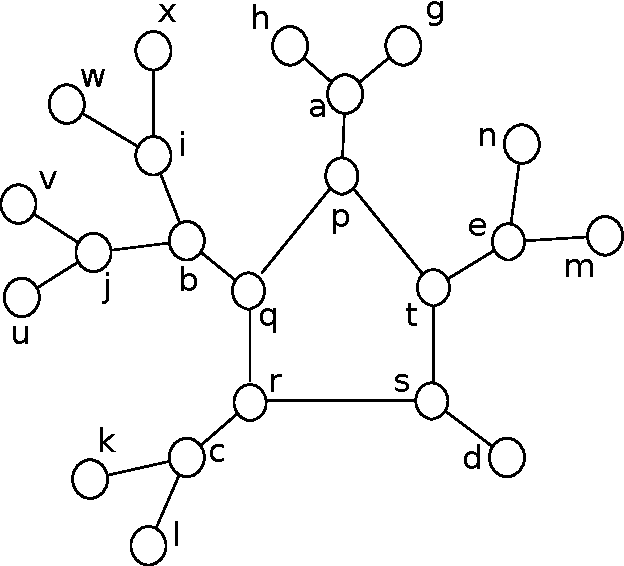
\includegraphics[scale=0.4]{pent}
\caption{Pentagon $pqrst$}
\label{fig:pent}
\end{center}
\end{figure}

\lipsum[1]

\section{SECTION NAME}
\lipsum[2]

\begin{table}
\centering
\begin{tabular}{| c | c |}
\hline
{\bf item 1} & {\bf item 2} \\ \hline
%
abcde & 5 \\ \hline
%
pqrst & 4 \\ \hline
\end{tabular}
\caption{A sample table}
\label{table:1}
\end{table}


\chapter{CHAPTER NAME}

%Replace \lipsum with text.
% You may have as many sections as you please. This is just for reference.

\section{SECTION NAME}
\lipsum[2]

\section{SECTION NAME}
\lipsum[3]

\section{SECTION NAME}
\lipsum[2]

\chapter{Work Done}

%Replace \lipsum with text.
% You may have as many sections as you please. This is just for reference.

\section{Sensor Tile Kit}

% TODO: Add android code screenshot that shows the limitation
In section \ref{ch1-intro-android}, we explained how Android limits the sensor data sampling rate to around 200Hz, which is good enough for monitoring device movements, such as tilt, rotation etc.
% TODO: Fix this line
but is low for our goal to use it as an microphone since human audible frequencies lie in the 20Hz to 20kHz range.
To explore what could be done if we had access to high frequency sensor data, we tried a specialized sensor board - the SensorTile by STMicroelectronics.

The SensorTile is a tiny, square-shaped IoT module that packs powerful processing capabilities leveraging an 80 MHz microcontroller, a Bluetooth low energy connectivity based on BlueNRG-MS network processor as well as a wide spectrum of motion, such as a triaxial accelerometer, gyroscope, magnetometer, and environmental sensors, such as pressure, humidity and temperature and even a digital microphone. \cite{stkit}

Figure \ref{fig:sensortilekit} shows the contents of the SensorTile kit.

\begin{figure}[H] \begin{center}
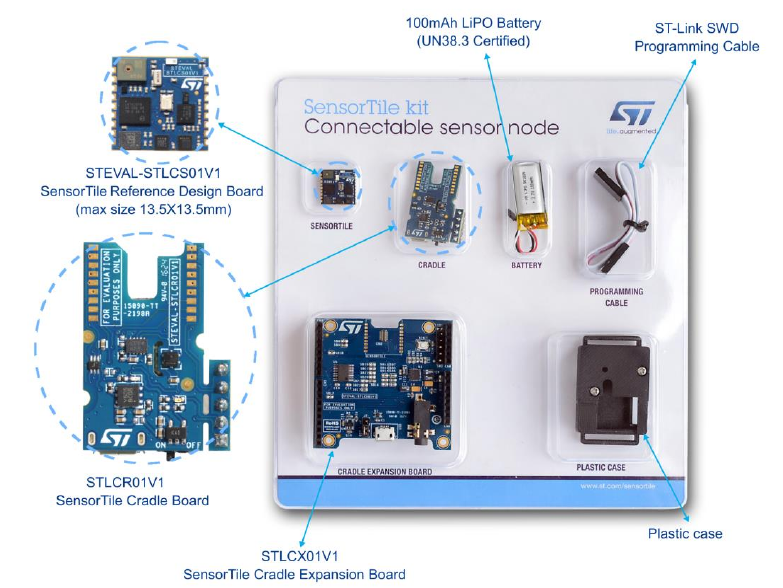
\includegraphics[scale=0.6]{sensortilekit}
\caption{SensorTile Development Kit}
\label{fig:sensortilekit}
\end{center} \end{figure}

\newpage

Figure \ref{fig:sensortile} shows position of main components of the SensorTile board, and Table \ref{table:sensortile} lists their description. \cite{stkitmanual}

\begin{figure}[H] \begin{center}
% \begin{wrapfigure}{l}{0.5\textwidth}
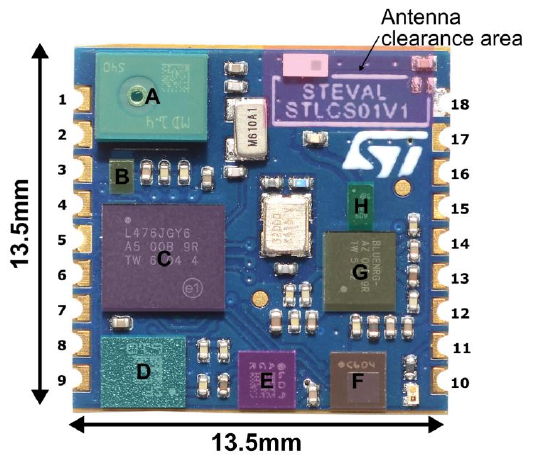
\includegraphics[scale=0.5]{sensortile}
\caption{SensorTile Main Components}
\label{fig:sensortile}
% \end{wrapfigure}
\end{center} \end{figure}

\begin{table}[H]
\centering
\begin{tabular}{@{}|c|l|p{0.55\linewidth}|@{}}
\hline
\toprule
{\bf Reference} & {\bf Device} & {\bf Description} \\ \hline
\midrule
A & MP34DT04      & MEMS audio sensor digital microphone \\ \hline
B & LD39115J18R   & 150 mA low quiescent current low noise LDO 1.8 V \\ \hline
C & STM32L476 MCU & ARM Cortex-M4 32-bit microcontroller \\ \hline
D & LSM6DSM       & iNEMO inertial module: low-power 3D accelerometer and 3D gyroscope \\ \hline
E & LSM303AGR     & Ultra-compact high-performance eCompass module: ultra-low power 3D accelerometer and 3D magnetometer \\ \hline
F & LPS22HB       & MEMS nano pressure sensor: 260-1260 hPa absolute digital output barometer \\ \hline
G & BlueNRG-MS    & Bluetooth low energy network processor \\ \hline
H & BALF-NRG01D3  & 50 Ω balun with integrated harmonic filter \\ \hline
\bottomrule
\end{tabular}
\caption{SensorTile Main Components}
\label{table:sensortile}
\end{table}

\newpage

By default, the SensorTile comes loaded

\newpage
\section{Android App}
\lipsum[1]

\newpage
\section{Analysis \& Results}
\lipsum[1]


\chapter{Conclusion}

\lipsum[2]


\chapter{Conclusion}

\lipsum[2]

\bibliographystyle{plain}
\bibliography{biblio}

% \appendix
% \chapter{CHAPTER NAME}

\section{SECTION NAME}
\lipsum[1]

\section{SECTION NAME}
\lipsum[2]

\end{document}

